\chapter{Use-case analysis}\label{chap:use_cases}
The introduction argued that validating properties on input parameters becomes expensive when a data structure (such as arrays), certain data types (such as byte sequences) or a range of values have to be iterated. It showed examples for such properties and identified logical formulas containing universal quantification as amenable for distributed assertion checking. As a matter of fact, the same is also valid for existential quantification, even though its negation has a different notion than that of its universal counterpart. The difference between the two is addressed later in this chapter. \\
The following section formally defines a set of applicable logical formulas for the first implementation of this approach. Given this set, section \secref{sec:examples} gives some more in-depth examples with their respective time complexity. \todo{General cost analysis?}

\section{Definition of a set of logical formulae}\label{sec:formulae}
As already mentioned, formulas containing universal and existential quantification are interesting use-cases. Predicate variables are, for now, limited to the primitive data types supported by the respective virtual machines (VM). Besides the basic logical, numerical and relational operators of predicate logic, the formula may contain any operation that is built into the VM.
\begin{align*}
    t &::= \text{primitive data types (existing in the blockchain VM)} \\
    \sigma &::= \forall \mid \exists \\
    \Theta &::= \Phi \mid \sigma (x:t) \Theta \\
    \Phi,\Psi &::= \neg\Phi \mid \Phi \Rightarrow \Psi \mid \Phi\wedge\Psi \mid
    				\Phi\vee\Psi \mid \Phi \oplus \Psi \mid M \rho N \\
    \rho &::= < \mid > \mid \le \mid \ge \mid = \mid \ne \\
    M, N &::= x \mid c \mid M \odot N  \mid f (\overline M) \\
    \odot &::= +\mid -\mid * \mid / \mid \% \\
    c &::= \text{constants: numbers, strings, } \top, \bot \\
    f &::= \text{operations (existing in the blockchain VM)}
\end{align*}
\begingroup\vspace*{-\baselineskip}
\captionof{figure}{Set of logical formulas amenable to distributed assertion checking (based on \cite{thiemann_2020})}
\vspace*{\baselineskip}\endgroup

\secref{} goes into more detail about what this set comprises of concretely for assertions executed on Tezos, and which extensions to Michelson and the VM are necessary in order to facilitate the assertion examples given previously and in the following section.
\todo{Secref}

\section{Interesting formulas and special cases}\label{sec:examples}
The following use-cases are picked from \cite{bernhardt_veigel_2020}, which contains a more comprehensive collection of formulas and properties that can be checked using the proposed approach. The selection of examples demonstrates different meanings of their negations and special cases, which emerge from different compositions of quantification, and discusses possible implications thereof.

\subsection{Two numbers are coprime}\label{sec:coprime}
The greatest common divisor ($gcd$) of two non-zero integers $a$ and $b$ is the largest integer that divides both evenly \cite{hardy2008introduction}. A more specific $gcd$-problem is finding two numbers which are coprime, meaning their greatest common divisor is one, i.e., $gcd(a, b) = 1$ \cite{hardy2008introduction}. In order to verify that two numbers are coprime, it has to be checked that there exists no $gcd > 1$, which can be expressed in the following formula in predicate logic:
\begin{equation}\label{eq:coprime-universial}
    (\forall n : int) (2 \le n \le \min(a,b)) \Rightarrow \neg((a \mathbin{\%} n) = 0 \land (b \mathbin{\%} n) = 0)
\end{equation}
Assuming constant time for calculating the two remainders, checking whether two numbers satisfy this property takes linear time, i.e. $\mathcal{O}(n)$, and depends on the size of the smaller number. When checking the assumption through a distributed effort instead, the validators consider its negation:
\begin{equation}\label{eq:coprime-existential}
    (\exists n : int) (2 \le n \le \min(a,b)) \land (a \mathbin{\%} n) = 0 \land (b \mathbin{\%} n) = 0
\end{equation}
If, within the given domain, this condition is true for a random value for $n$, the respective validator has found a counterexample.

\subsection{Heap property}
Heaps are data structures based on trees and can appear in two varieties: min and max heaps. Both can be represented as binary trees and have to satisfy the heap property \cite{dict_heap}: in a max heap, any given node holds a value lower or equal than that of its parent, whereas in a min heap, it is greater or equal \cite{dict_heap_property}. Binary heaps are often implemented as an array, with the root of the tree stored at index 0. The relatives of a node \texttt{k} can be accessed as follows \cite{dict_binary_heap}:
\begin{lstlisting}[language=Solidity, numbers=none, caption=Access a binary heap in array representation \cite{bernhardt_veigel_2020}]
heap_array[(k-1)/2] // Get parent of node k
heap_array[(k*2)+1] // Get left child of node k
heap_array[(k*2)+2] // Get right child of node k
\end{lstlisting}
The min heap property for a binary heap stored in an array $a$, for instance, can be expressed in predicate logic with the following formula:
\begin{equation}\label{eq:heap-unversial}
  (\forall k : int) (1 \le k < |a|) \Rightarrow a[\lfloor(k-1)/2)\rfloor] \le a[k]
\end{equation}
The time complexity of checking whether $a$ satisfies the heap property depends on how the array is allocated. If it is dynamically sized, it takes $\mathcal{O}(n)$ in the size of the array, otherwise it takes constant time, i.e. $\mathcal{O}(1)$.  Similarly to the previous examples, counterexamples can be identified by considering the formula's negation:
\begin{equation}\label{eq:heap-unversial-neg}
  (\exists k : int) (1 \le k \le |a|) \land a[\lfloor(k-1)/2)\rfloor] > a[k]
\end{equation}

\section{Existential quantifier and proofs of validity}\label{sec:existential}
The examples given so far in this thesis used universal quantification and required a search for counterexamples in order to check if some assumption about an input parameter is true. However, the same cannot be applied to existential quantifiers. Consider a contract expecting two intersecting sets of integers, represented as arrays. The assumption, that the intersection of the sets is not empty, i.e., $U \cap V \neq \emptyset$, can be expressed by
\begin{equation}\label{eq:intersect}
  (\exists i, \exists j) (0 \le i < |u|) \land (0 \le j < |v|) \Rightarrow u[i] = v[j]
\end{equation}
Consider its negation:
\begin{equation}\label{eq:intersect_neg}
  (\forall i, \forall j) (0 \le i < |u|) \land (0 \le j < |v|) \land u[i] \neq v[j]
\end{equation}
If the condition is true for random values of $i,j$, it does not produce a counterexample, but it rather produces a proof for the validity of the assumption. In that case, the validator finding such a proof should publish an approval instead of a veto to the network and the normal execution of the contract can proceed. Thus, the two quantifiers essentially represent two different modi of assertion checking that the executors need to be aware of. \todo{If I pick this up again in a later chapter, ref.}\\
Concerning the complexity of this test, the property can be checked in $\mathcal{O}(|u|*|v|)$. By considering the cardinality of their union $n = |u|+|v|$, one can derive that the worst case occurs when both sets have the same size, i.e., $|u| = |v| = n/2$. This leads to a quadratic complexity $\mathcal{O}(n/2 * n/2) = \mathcal{O}(n^2/4) = \mathcal{O}(n^2)$.

\section{Nested quantification}
The previous example showed that universal and existential quantification have to be handled differently. However, further special cases caused by nested quantification have to be considered as well. A nesting of the same type of quantifier, e.g. $\forall i \forall j$ can be considered as trivial. They can be handled by generating a random value for each predicate variable and checking for a counterexample or proof respectively. It becomes less trivial though, if the nesting contains both universal and existential quantifiers. This section examines the case of $\exists i \forall j$ on the basis of a contract that expects a solution for a boolean satisfiability problem (SAT). Another instance of this use-case is also used to show that properties expressed with the nesting $\forall i \exists j$ cannot be checked with the proposed approach for distributed assertion checking offhand.

\subsection{Boolean satisfiability problem}\label{sec:sat}
Instances of SAT problems consist of a formula $F$ in propositional logic, and determine if there exists a variable assignment $\mathcal{A}$ to the values $true$ or $false$, s.t. the formula is satisfied ($\mathcal{A}(F) = 1$) \cite{Biere2009}. Modern SAT-solvers expect $F$ to be in conjunctive normal form (CNF), i.e., a conjunction of a set of clauses, where clauses are disjunctions of variables or their negations (called literals) \cite{cnf_math_encycl}. While finding an assignment $\mathcal{A}$ that satisfies $F$ is a NP-complete problem \cite{Biere2009}, verifying whether a given assignment satisfies the formula takes $\mathcal{O}(n*m)$, where $n$ is the number of clauses and $m$ the number of variables (in the worst case, every variable is present as a literal in each clause). In the case of k-SAT problems, where each clause contains at most k literals \cite{Biere2009}, the complexity is reduced to $\mathcal{O}(n)$.

\subsubsection{Encoding of variables, literals and clauses}
A SAT problem can be represented as a list of clauses $c$ and a variable assignment $\mathcal{A}$. To avoid having to handle the variables and their literals as strings and thus optimize runtime and memory consumption, an encoding scheme taken from this blogpost\cite{sabablog} is used: \\
Variables are encoded by a unique number starting from $0$ to $n-1$, where $n$ is the total number of variables. The positive and negative literals of a variable with id $x$ are encoded by the function
\begin{align*}
encode(x) =
\begin{cases}
  $2x$  & \text{if x is present as a positive literal}\\
  $2x+1$ & \text{if x is present as a negated literal}\\
\end{cases}   
\end{align*}
Consequently, checking whether a literal $y$ is positive or negative is a simple bit-wise $AND$ operation:
\begin{align*}
\texttt{isPositive(y) = y \& 1 == 0}
\end{align*}
As already mentioned, $F$ can be represented as a list of clauses, and each clause in turn can be represented as a list of literals. Consider the following boolean formula and variable assignment:
\begin{align*}
F = (A \vee B) \wedge (B \vee \neg C) \text{, } \mathcal{A} = \{A \rightarrow false, B \rightarrow true, C \rightarrow false\}
\end{align*}
Following the encoding of variables given above, the list of variables $v=[A,B,C]$ occurring in $F$ is encoded as $v_{enc} = [0,1,2]$. $F$ is thus represented by the encoding $F_{enc} = [[0,2],[2,5]]$. Since the encoding of variables corresponds to their index in the list of variables, $\mathcal{A}$ can be passed as a list of booleans that maintains the same order of variables: $\mathcal{A}_{enc} = [False, True, False]$. If the blockchains VM supports a respective data type, $\mathcal{A}$ can alternatively be represented with a more efficient bitarray. Lastly, the variable encoding $x$ of a literal $y$ is obtained by dividing its encoding by two, which corresponds to a bit-wise shift to the right:
\begin{align*}
\texttt{decode(y) = y >> 1}
\end{align*}

\subsection{Satisfiability in predicate logic - DNF}\label{sec:dnf}
In opposition to the statement that modern SAT solvers expect $F$ to be in CNF, consider a contract that expects a SAT problem in disjunctive normal form (DNF) and a proposed assignment, both encoded as described above. A boolean formula in DNF is a disjunction of conjunctions \cite{dnf_math_encycl}. Assuming that $F$ is a k-SAT instance, the assumption that $\mathcal{A}$ satisfies $F$ can be expressed in predicate logic as follows:
\begin{gather*}\label{eq:dnf_sat}
\begin{aligned}
(\exists i : int, \forall j : int) (0 \leq i < |F|) \wedge (0 \leq j < k) &\Rightarrow ((isPositive(F[i][j]) \wedge \mathcal{A}[decode(F[i][j])]) \\
&\vee (\neg isPositive(F[i][j]) \wedge \neg \mathcal{A}[decode(F[i][j])])))
\end{aligned}
\end{gather*}
With single quantification, we so far considered the negation of the formula in order to identify counterexamples (or proofs). However, by checking some literal in some clause, the validator cannot make a statement about the validity of the property, as the clauses have to be examined as a whole in order to verify that the conjunction evaluates to true. Consequently, the distribution can only take place on the level of clauses, but not on the level of literals. Each validator thus has to check all literals of one random clause and produce a proof of validity if all of them satisfy the property. This implies that the formula does not have to be negated. \\
Besides having a distinct transformation, this case also has to be handled differently during the compilation process; instead of translating both quantifiers into a random generator, the universal quantifier has to be translated into a loop, cf. \lstref{lst:rand_loop}.
\begin{lstlisting}[label=lst:rand_loop, numbers=none, caption=Translation of an assertion for a DNF SAT problem in pseudo-code]
i = random(0, size(F))
for (j : [0..k)):
	check(...)
\end{lstlisting}
In the case of k-SAT instances, the validators still only have to be paid a constant amount of gas, albeit with a factor $k$. If the number of literals in a clause is not constant, the loop will introduce a linear cost factor for each validator.

\subsection{Satisfiability in predicate logic - CNF}
Unfortunately, the same cannot be applied for the reverse quantification nesting. Consider the same contract, but instead of expecting $F$ in DNF, it expects it to be in CNF. The domain restrictions and open formula remain the same, but the quantifiers are in reverse order:
\begin{gather*}\label{eq:cnf_sat}
\begin{aligned}
(\forall i : int, \exists j : int) (0 \leq i < |F|) \wedge (0 \leq j < k) &\Rightarrow ((isPositive(F[i][j]) \wedge \mathcal{A}[decode(F[i][j])]) \\
&\vee (\neg isPositive(F[i][j]) \wedge \neg \mathcal{A}[decode(F[i][j])])))
\end{aligned}
\end{gather*}
Again, the validator has to check the whole clause in order to know whether it evaluates to true. Due to existential quantification, however, the literals in the clauses cannot be checked independent of each other. A single literal evaluating to false does not make the whole clause evaluating to false. Although technically possible, it requires a more sophisticated compiler that translates this nesting into the following code structure:
\begin{lstlisting}[label=lst:rand_loop_dependent, numbers=none, caption=Translation of an assertion for a CNF SAT problem in pseudo-code]
i = random(0, size(F))
for (j : [0..k)):
	if check(...):
		assert(true)
assert(false)
\end{lstlisting}

\subsection{Further nesting}
Nesting is, of course, not limited to two quantifiers only. Generally, formulas containing no quantification alterations within the nesting benefit the most from distributed assertion checking, as each quantifier can be translated into a random generator. On the other hand, formulas with a quantifier alteration early in the order of quantifiers benefit the least, because starting from the first alteration, the following quantifiers are translated to loops.\\
To substantiate this argument, consider two variations of a contract that expect a list of boolean formulas in DNF, and an assignment $\mathcal{A}$. The first one checks, whether $\mathcal{A}$ satisfies at least one $F$, the other one checks if all $F$ are satisfied. This can be expressed by nesting quantifications as follows: 
\begin{itemize}
\item $\exists f \exists i \forall j$
\item $\forall f \exists i \forall j$
\end{itemize}
In the first case, each validator picks a random clause from a random $F$ and checks if all literals evaluate to true. In the second case, checking a random clause in isolation cannot disprove the satisfiability, hence the validator has to check all clauses in a loop. The same reasoning can be done for the reverse order, i.e. $\forall\forall\exists$ and $\exists\forall\exists$.

\subsection{Restriction of use-cases}\todo{Better title?}
The examples given in this chapter have shown that, depending on the type and order of quantification, not all properties can be checked in the same way and need different modi of assertion checking. This increases the complexity and requirements for a implementation of this approach; therefore, for a first iteration, this thesis focuses on providing the fundamentals and implementation for assertions using universal quantification only.

\section{Cost analysis}\label{sec:usecase_cost}
In order to be able to evaluate whether distributed assertion checking can indeed lower the cost in comparison to a local verification, the cost of checking a formula on the blockchain needs to be formalized. Since this thesis describes an implementation of the approach on the Tezos blockchain, the following costs refer to that specific gas model, s.t. the results of the cost analyses are comparable (Tezos and its gas model are described in more detail in \secref{sec:tezos}). \\
According to the gas model, the total gas consumption of a transaction $T(src,\, dst=C,\, arg, \, ...)$ to an originated contract $C(storage, \, parameter\, type, \, code)$ is calculated by \eqref{eq:gas_transaction}, where $I$ is the set of internal operations:
\begin{align}\label{eq:gas_transaction}
\begin{split}
GasConsumed(T) = \quad &base \, amount \\
+& \, gasRead(code) \\
+& \, gasRead(storage) \\
+& \, gasDeserialize(storage, \, arg) \\
+& \, gasParseType(parameter \, type, \, storage) \\
+& \, gasParseData(storage, \, arg) \\
+& \, gasParseCode(code) \\
+& \, gasInterpret(code, \, arg, \, storage) \\
+& \, gasUnparse(storage) \\
+& \, gasSerialize(storage) \\
+& \, gasWrite(storage) \\
+& \, \sum_{i \in I} GasConsumed(i)
\end{split}
\end{align}
Assuming that the storage is never increased, the amount of gas returned by the cost functions independent of the argument, i.e., the parameter value, remain constant for each $T$. The cost functions for the deserialization, parsing and interpretation, however, are functions of $arg$ that grow strictly monotonic with increasing sizes of $arg$. \\
Consider the following simple contracts --- they do not do anything useful, but can be used to approximate the amplification of costs with regard to $arg$. Contract \texttt{Foo} takes an integer, whose byte sequence does not increase significantly with higher values, thus the increase in overall cost is mainly accounted for by interpretation cost. Contract \texttt{Bar}, on the other hand, executes similar operations but expects a list of integers, which causes noticeably higher deserialization and parsing costs with increasing input size. 
\begin{lstlisting}[numbers=none, language=Solidity, caption=Simple dummy contract executing a loop]
contract Foo {
  function foo (int a) public {
    for (uint i = 0; i < a; i++) {
      assert(a == a)
	}
	// ...
  }
}
\end{lstlisting}
\begin{lstlisting}[numbers=none, language=Solidity, caption=Simple dummy contract iterating over a list]
contract Bar {
  function bar (int [] b) public {
    for (uint i = 0; i < b.length; i++) {
      assert(b[i] = b[i])
	}
	// ...
  }
}
\end{lstlisting}

\figref{fig:use_case_cost} shows the reported gas consumption of transactions calling the dummy contracts on the Delphinet test network running the protocol 007 Delphi \cite{tezos_docs}. As to be expected, the gradient of the cost function in the case of \texttt{Bar} is higher due to additional serialization and parsing costs, namely $\frac{dx}{dy} = 16$ compared to $\frac{dx}{dy} = 6$ for \texttt{Foo}.
\begin{figure}[t]
\centering
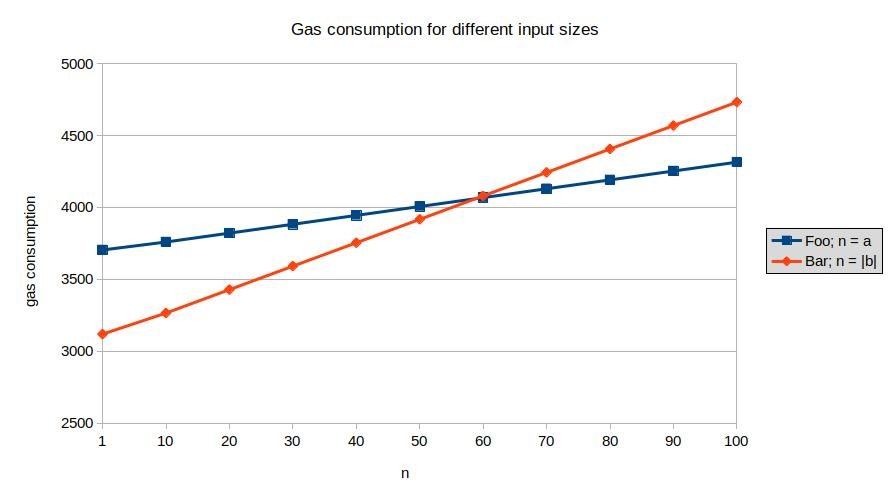
\includegraphics[width=0.9\linewidth]{figures/2-use_cases/cost_analysis}
\caption{Gas consumption of transactions calling \texttt{Foo} and \texttt{Bar} for increasing input sizes}
\label{fig:use_case_cost}
\end{figure}

A repeated cost analysis is carried out in \secref{sec:cost_analysis_distributed} in order to assess whether, or how, distributed assertion checking, as described in the following chapters, can achieve a reduction of these costs.